% Can Decision Models Replace Tool Calling for Coding Agents?
% Main result: the coding-harness ablation (results/harness_v2, results/harness_v2_300). Supporting evidence from
% the earlier studies (selection at scale, SynthHolster, pre-registered test, real trajectories, argument ceiling).
\documentclass[11pt]{article}
\usepackage[T1]{fontenc}
\usepackage[utf8]{inputenc}
\usepackage{lmodern}
\usepackage{microtype}
\usepackage[margin=1in]{geometry}
\usepackage{amsmath,amssymb}
\usepackage{booktabs}
\usepackage{tabularx}
\usepackage{multirow}
\usepackage{graphicx}
\usepackage{xcolor}
\usepackage{enumitem}
\usepackage{caption}
\usepackage{subcaption}
\usepackage{fvextra}
\usepackage{tikz}
\usetikzlibrary{positioning,arrows.meta,shapes.geometric,fit,calc}
\usepackage[numbers,sort&compress]{natbib}
\usepackage[colorlinks=true,linkcolor=blue!50!black,citecolor=blue!50!black,urlcolor=blue!50!black]{hyperref}

\setlist{itemsep=2pt,topsep=3pt}
\captionsetup{font=small,labelfont=bf}
\setlength{\emergencystretch}{3em}
\let\oldus\_\renewcommand{\_}{\oldus\discretionary{}{}{}}
\newcommand{\msd}{MSD1}
\newcommand{\cmark}{\textcolor{green!45!black}{\ding{51}}}
\newcommand{\todo}[1]{\textcolor{red!70!black}{[TODO: #1]}}
\newcommand{\expl}{\textsc{exploratory}}
\newcommand{\conf}{\textsc{confirmatory}}
\usepackage{pifont}

\usepackage{longtable}

\title{\textbf{Can Decision Models Replace Tool Calling for Coding Agents?}}
\author{Aziz Muminov \and Alexandra Ilyina}
\date{Preprint draft --- 27 October 2026}

\begin{document}
\maketitle

\begin{abstract}
Coding agents increasingly carry large tool catalogs, and every request re-sends every tool definition. We
test whether a \emph{decision model} (DM), a model that returns a probability for each of a set of
caller-supplied options without generating text, can take the catalog's place. We built a sandboxed
coding-agent benchmark: an unmodified open-source agent works on 30 Python repositories whose hidden tests
require facts available only through a fictional company's internal catalog of 100 or 300 tools. Instead of
the catalog, the agent gets one universal tool: it states what it needs, a DM picks the matching tools, and the
agent calls one. Across 1{,}260 runs with two LLMs, the universal tool matched loading every definition
(98--99\% vs.\ 97--99\% success on tasks that need the catalog) while reading 81\% less context per run with
100 tools and 92--93\% less with 300, at a quarter to an eighth of the cost. Two conditions matter. The agent
must be told which services exist: without a one-line list it sometimes never searches. And tools must be
selected when the need arises: choosing them upfront from the task prompt solved 14\% of tasks whose needs
appear mid-task. The DM does not replace the agent's own calls (on a real coding session it predicted the next
tool less often than ``always use the shell''); it replaces the catalog.
\end{abstract}

%=====================================================================
\section{Introduction}\label{sec:intro}
%=====================================================================

A coding agent acts through tools: a shell, file reading and editing, search, and, increasingly, the tools of
every service its organization exposes through protocols such as MCP~\citep{mcp}: issue trackers, CI systems,
configuration services, documentation, databases. Each tool comes with a definition (a description and a
parameter schema) that the agent's LLM reads on every request, whether or not the tool is used. In the agent
session in which this paper's experiments were built, 51 always-loaded tool definitions took about
59{,}000 tokens, 93\% of the first request, and were re-sent with each of 435 requests; the agent used 10 of
them (\S\ref{sec:overhead}). The coding agent we test documents the same problem: tool servers ``tend to add a
lot of tokens and can easily exceed the context limit''~\citep{opencode}.

\emph{Decision models} (DMs), released by several vendors in 2026~\citep{typesafejev,msd1,openrouterdecisions},
are built for choices. A DM reads a state and answers typed questions (yes/no, pick one of these options, give a
score) with a probability per option, in one forward pass, with no generated tokens, in well under a second
and for about \$0.04 per million input tokens. Finding the right tool in a catalog is such a choice. We
therefore replace the catalog with a \emph{universal tool} (Figure~\ref{fig:universal}): the agent keeps its
core coding tools and gets two more, \texttt{find\_tool(intent)}, which a DM resolves against the full catalog
at the moment the agent asks, and \texttt{call\_tool(name, arguments)}. The catalog leaves the prompt; the LLM
still writes the intent, the arguments and the code.

\begin{figure}[t]
\centering
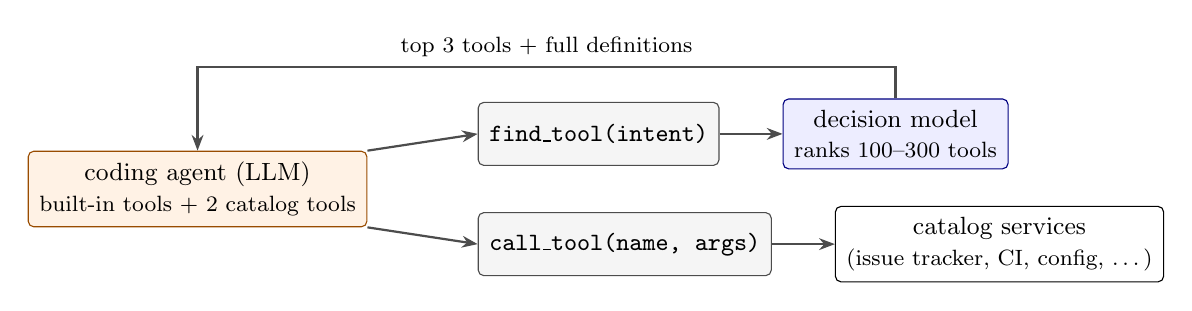
\begin{tikzpicture}[font=\small, node distance=5mm and 8mm,
  box/.style={draw, rounded corners=2pt, align=center, inner sep=4pt, minimum height=8mm, fill=white},
  dm/.style={box, fill=blue!7, draw=blue!50!black}, llm/.style={box, fill=orange!10, draw=orange!60!black},
  outb/.style={box, fill=gray!8, draw=gray!60!black}, arr/.style={-{Stealth[length=2mm]}, thick, draw=gray!60!black}]
\node[llm] (agent) {coding agent (LLM)\\ \footnotesize built-in tools + 2 catalog tools};
\node[outb, right=14mm of agent, yshift=7mm] (find) {\texttt{find\_tool(intent)}};
\node[dm, right=of find] (dm) {decision model\\ \footnotesize ranks 100--300 tools};
\node[outb, right=14mm of agent, yshift=-7mm] (call) {\texttt{call\_tool(name, args)}};
\node[box, right=of call] (svc) {catalog services\\ \footnotesize (issue tracker, CI, config, \dots)};
\draw[arr] (agent.north east) -- (find.west);
\draw[arr] (find) -- (dm);
\draw[arr] (dm.north) -- ++(0,4mm) -| node[pos=0.25, above, font=\footnotesize]{top 3 tools + full definitions} (agent.north);
\draw[arr] (agent.south east) -- (call.west);
\draw[arr] (call) -- (svc);
\end{tikzpicture}
\caption{The universal tool. The agent's prompt holds two short tool definitions instead of the catalog; the
decision model resolves each stated intent at the moment the agent needs it.}
\label{fig:universal}
\end{figure}

Whether this works is a question about the whole agent loop, not about single calls: the agent must decide to
look for a capability it cannot see, describe it well enough, and use what comes back. We therefore built a
coding-agent benchmark for it (\S\ref{sec:bench}). An unmodified open-source coding agent~\citep{opencode} runs
in an operating-system sandbox on 30 small Python repositories. Their hidden tests require values that only a
fictional company's internal services return (a production configuration value, a feature flag, a CI
threshold, an API contract), through a catalog of 100 or 300 realistic tools; some needs appear only after a
first lookup, and some values do not exist at all. We compare five ways of exposing the catalog, from none to
all definitions, with two LLMs, in 1{,}260 runs. We find:
\begin{itemize}
\item \textbf{The universal tool matches loading the whole catalog.} With a one-line list of the services the
catalog covers, it passed 112 of 114 runs that need the catalog against 113 for native tool calling at 100
tools, and 75 of 76 against 74 at 300 tools (\S\ref{sec:catalog}, \S\ref{sec:scale}).
\item \textbf{It removes most of the context.} The largest prompt fell from 61--65k to 10--12k tokens at 100 tools
and from 169--178k to 10--12k at 300; the context read per run fell by 81\% and 92--93\%, the cost per run to
a quarter and an eighth.
\item \textbf{Two design choices decide whether it works.} Without the service list, agents sometimes never
search for a capability they do not know exists (\S\ref{sec:breaks}). Choosing tools once from the task
prompt instead of at the moment of need solved 14\% of tasks whose needs appear mid-task.
\item \textbf{No condition invented a value}: where the value did not exist, every run abstained.
\end{itemize}
The DM's role is selection only. A DM cannot write arguments, and on the tool decisions of a real coding
session it predicted the agent's next tool less often than always choosing the shell (\S\ref{sec:calls}): it
replaces the catalog, not the agent's tool calls.

\paragraph{Contributions.} (i)~A sandboxed coding-agent benchmark for tool catalogs: an unmodified open-source
agent, a fictional 100/300-tool catalog, 30 tasks with hidden tests, five tool-exposure conditions, and
false-positive and abstention accounting. (ii)~Evidence from 1{,}260 runs that a DM-backed universal tool
preserves task success at a fraction of the context, and grows more valuable as the catalog grows.
(iii)~An analysis of its failure modes and a design recipe. (iv)~A measurement of what tool definitions cost
in a real coding session, and of why a DM cannot take over the agent's own calls.

%=====================================================================
\section{Background and related work}\label{sec:background}
%=====================================================================

\paragraph{Decision models.} We use OpenRouter's Decisions API~\citep{openrouterdecisions}: a request carries a
\emph{state} (text or JSON) and named questions of type yes/no, \texttt{choice} (one of named options, each
with a free-text description; returns a distribution) or \texttt{score}. We evaluate
Microsoft-Decision-1 (\msd{}), a post-trained Qwen3.5-9B~\citep{msd1}, and TypeSafe Jev~1.14~\citep{typesafejev}.
In our runs both rejected a \texttt{choice} with more than 255 options, and \msd{} requests beyond 32k tokens.
The Artificial Analysis Decision Index~\citep{aa2026decisionindex} and an analysis of it~\citep{olson2026decision}
compare DMs with LLMs on standalone tasks and find them about even on tool-call routing; neither places a DM
inside an agent.

\paragraph{Too many tools.} Retrieving tools before generation is the standard answer to large
catalogs~\citep{qin2023toolllm,oats2026}, and \citet{selection2026retrieval} find that selecting a tool is
largely retrieval while recognizing that none applies is the hard part. Agent harnesses increasingly defer
tool definitions and load them on demand by keyword search; the agent that built this paper did so for some
of its tools. We test a learned, semantic version of this idea inside an unmodified coding agent, and measure
its effect on end-to-end task success.

\paragraph{Deciding when to call.} When2Call~\citep{ross2025when2call}, SMART~\citep{qian2025smart}, ``To Call or
Not to Call''~\citep{tocall2026} and Probe\&Prefill~\citep{sun2026probe} study whether an LLM should call a tool at
all. Coding agents mid-task almost always act, so we do not study this gate here.

\paragraph{Benchmarks.} Tool-calling benchmarks such as BFCL~\citep{patil2025bfcl} score single calls with small
menus; agentic benchmarks score task completion~\citep{yao2024taubench,mcpatlas2026,toolathlon2025}, and their
evaluators are themselves noisy~\citep{audit2026}. We therefore built tasks scored by hidden unit tests, in a
fictional organization whose tools no model can have seen.

%=====================================================================
\section{Where does tool calling cost context?}\label{sec:overhead}
%=====================================================================
We parsed the full transcript of the coding session in which this paper's experiments were built (one agent,
32 user requests, 453 tool calls in 395 decisions, 435 LLM requests). It records the prompt the agent ran
with. Its 51 always-loaded tool definitions took about
202{,}000 characters, about 58{,}900 tokens (calibrated against the first request, 63{,}454 tokens before
any conversation), and were re-sent with every request: about 25 million of the 162 million context
tokens the session read (16\%). Two items alone cost about 39{,}000 tokens per request and were called once between them: a publishing tool (17{,}400) and 30 cloud-session tools (21{,}300). The agent used 10 of the
51. Measured per tool, real definitions averaged about 1{,}150 tokens (MCP tools: about 700), against about
150 in BFCL.

Prompt caching makes these tokens cheap but not free: at the session model's cached-read price (\$0.20 per
million) they cost about \$5 of a \$60 session, and they occupy the context window on every request. Without
caching (one-off calls, tool lists that change between requests, low traffic) the same definitions are billed
at full input price: for 100 tools of 700 tokens, about \$280 per thousand requests at \$4 per million input
tokens, against about \$0.50 per thousand DM calls that each select among 200 tools (App.~\ref{app:support}).

%=====================================================================
\section{A coding-agent benchmark for tool catalogs}\label{sec:bench}
%=====================================================================
The benchmark asks whether an agent that cannot see the catalog still finds and uses the tools it needs, and
what each way of exposing the catalog costs in context.

\paragraph{Harness.} We run opencode~\citep{opencode} (v1.19.4), an open-source coding agent, unmodified and
headless. It keeps its built-in tools (read, edit, glob, grep, list, a to-do list, and a shell restricted to
running \texttt{pytest}) in every condition; web access is off. The catalog is served by our MCP server over
local HTTP.

\paragraph{Sandbox.} A first pilot with harness-level permissions only was invalid: the agent read the hidden
tests and answer files of its own task through absolute paths (App.~\ref{app:harness}). All reported runs
therefore execute as an unprivileged operating-system user with an empty environment, in a fresh copy of
the task. The experiment's files and the API key are readable only by root. The LLM is reached through a
local proxy that adds the key and admits only the two experiment models, and the catalog server runs as
root. We scanned every transcript for file access outside the task folder.

\paragraph{Catalog.} A fictional company with 12 internal services (issue tracker, CI, feature flags,
configuration, documentation and API-contract registry, warehouse, metrics, deployments, chat, on-call, code
search, package registry) exposes 100 tools (Table~\ref{tab:services}). Each has the shape of a real MCP tool,
a multi-paragraph description with parameters, return format, errors, limits and an example call, and averages
about 610 tokens, close to the MCP tools measured in \S\ref{sec:overhead}; the catalog totals about 61{,}000
tokens. A 300-tool catalog adds 20 services, several deliberately close to an original one (a support desk
beside the issue tracker, A/B experiments beside feature flags), for about 184{,}000 tokens. Every tool
answers deterministically from a per-task world file: the right tool with sensible arguments returns the
needed fact, anything else an empty list or \texttt{NOT\_FOUND}.

\paragraph{Tasks.} Thirty small Python repositories (Table~\ref{tab:tasks}), each scored by hidden tests:
\emph{control}~(6) bugs fixable from the repository alone; \emph{single}~(11) the code must use one value that
only a catalog tool returns (a production config value, a flag, a column width, a package version, an SLO
target, a service owner, a chat decision, a constant in another repository, a CI threshold); \emph{mid-task}~(7)
the first lookup (a ticket, a chat thread, a docs page, a CI log) points to a second service, so the second need
cannot be predicted from the prompt; \emph{contract}~(1) implement a parser from an API contract; and
\emph{absent}~(5) the value does not exist anywhere the agent can reach (a missing record, or a system not in
the catalog). Every value prompt ends with the same escape clause: if the authoritative value cannot be found,
leave it unchanged and add a \texttt{TODO: value not found} comment. The right outcome on absent tasks is to
abstain; changing the value is a fabrication. We validated every task: hidden tests fail on the original code
and pass with a reference solution.

\paragraph{Conditions.} Table~\ref{tab:hconditions}. In the two universal conditions the agent sees two tools
instead of the catalog (Figure~\ref{fig:universal}): \texttt{find\_tool(intent)}, for which \msd{} ranks
the catalog against the stated intent and returns the top three tools with their full definitions, and
\texttt{call\_tool(name, arguments)}. With 300 tools, \texttt{find\_tool} shortlists five tools from each half of
the catalog and decides among the ten (the 255-option limit). The \emph{service list} variant adds one line per
service to \texttt{find\_tool}'s description (App.~\ref{app:harness}).

\begin{table}[t]
\centering\small
\caption{Tool-exposure conditions. Built-in coding tools are present in all of them.}
\label{tab:hconditions}
\begin{tabularx}{\linewidth}{@{}l X@{}}
\toprule
Condition & What the agent sees of the catalog \\
\midrule
none & nothing (shows which tasks need the catalog) \\
native & every catalog tool with its full definition, in every request \\
filtered & the 5 tools \msd{} ranks highest for the task prompt, chosen once before the run \\
universal & \texttt{find\_tool} and \texttt{call\_tool}; no hint of what the catalog contains \\
universal + list & the same, plus a one-line list of the services the catalog covers \\
\bottomrule
\end{tabularx}
\end{table}

\paragraph{Models and runs.} Two LLMs drive the agent: DeepSeek~V4.1~Flash and GLM-5.3, both with 1M-token
context windows. Each of the 30 tasks ran under all five conditions with both models, three times (900 runs,
100 tools). We report pass rates with 95\% confidence intervals that resample whole tasks, exact McNemar tests
on runs paired by task, model and repeat, and the tokens and cost opencode records per request (its cost
matched the provider's bill within 1\%: \$8.84 for the 900 runs).

%=====================================================================
\section{Can a decision model replace the tool catalog?}\label{sec:catalog}
%=====================================================================
\begin{table}[t]
\centering\small
\caption{Main results, 100-tool catalog (30 tasks $\times$ 3 repeats per row). Pass rate over all tasks, with a
task-clustered 95\% CI; largest prompt and context read per run are means over runs.}
\label{tab:main}
\setlength{\tabcolsep}{4pt}
\begin{tabular}{@{}llccrrr@{}}
\toprule
Model & Condition & Pass rate [95\% CI] & Steps & Largest prompt & Context read / run & Cost / run \\
\midrule
DeepSeek & none & 0.367 [0.20, 0.53] & 7.0 & 8{,}193 & 50{,}537 & \$0.0049 \\
 & native & 1.000 [1.00, 1.00] & 7.2 & 64{,}536 & 460{,}805 & \$0.0266 \\
 & filtered & 0.789 [0.63, 0.92] & 8.0 & 11{,}919 & 89{,}322 & \$0.0080 \\
 & universal & 0.978 [0.94, 1.00] & 8.4 & 11{,}269 & 81{,}047 & \$0.0066 \\
 & universal + list & \textbf{1.000} [1.00, 1.00] & 8.0 & 12{,}297 & 88{,}417 & \$0.0067 \\
\midrule
GLM-5.3 & none & 0.367 [0.20, 0.53] & 6.7 & 6{,}866 & 42{,}714 & \$0.0040 \\
 & native & 0.989 [0.97, 1.00] & 5.4 & 60{,}631 & 324{,}141 & \$0.0233 \\
 & filtered & 0.789 [0.63, 0.92] & 6.3 & 9{,}873 & 60{,}699 & \$0.0058 \\
 & universal & 0.878 [0.78, 0.97] & 7.5 & 9{,}139 & 61{,}954 & \$0.0059 \\
 & universal + list & \textbf{0.978} [0.93, 1.00] & 6.6 & 9{,}593 & 60{,}028 & \$0.0055 \\
\bottomrule
\end{tabular}
\end{table}

\begin{figure}[t]
\centering
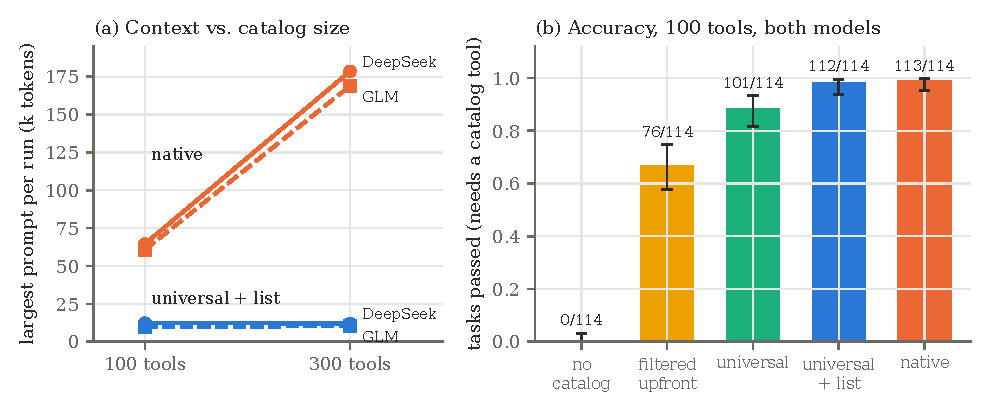
\includegraphics[width=\linewidth]{figures/fig_harness.pdf}
\caption{(a) The largest prompt of a run grows with the catalog when every definition is loaded and stays flat
with the universal tool (means over runs; 300-tool runs from \S\ref{sec:scale}). (b) Share of runs passed on
the 19 tasks that need a catalog tool (single, mid-task, contract), 100 tools, both models pooled, with
Wilson 95\% intervals.}
\label{fig:harness}
\end{figure}

\paragraph{The universal tool with a service list matches native.} On tasks that need a catalog tool it passed
112 of 114 runs, against 113 of 114 for native (Figure~\ref{fig:harness}b); paired by task, model and repeat,
one run passed only with the universal tool and two only with native ($p=1$). It read 81\% less context per
run (Table~\ref{tab:main}): the largest prompt fell from 61--65k to 10--12k tokens and the context read over a
whole run from 324--461k to 60--88k, at about a quarter of native's cost, for about one extra step per run (the
search).

\paragraph{Without the list, the universal tool loses some accuracy.} It passed 101 of 114 runs; against native
the paired difference is significant (0 vs.\ 12 discordant runs, $p=0.0005$), almost entirely through GLM
(0.878 overall). \S\ref{sec:breaks} shows why.

\paragraph{The tasks need the catalog, and the controls do not.} Without a catalog no run passed a task that
needs one (0 of 114); every control and absent task passed in every condition (Table~\ref{tab:cats}). No
control run touched the catalog.

\begin{table}[t]
\centering\small
\caption{Pass rate by task category, 100 tools, both models (6 runs per task and condition).}
\label{tab:cats}
\begin{tabular}{@{}lccccc@{}}
\toprule
Category (tasks) & none & native & filtered & universal & universal + list \\
\midrule
control (6) & 1.00 & 1.00 & 1.00 & 1.00 & 1.00 \\
single (11) & 0.00 & 1.00 & 0.97 & 0.94 & 1.00 \\
mid-task (7) & 0.00 & 0.98 & \textbf{0.14} & 0.79 & 0.95 \\
contract (1) & 0.00 & 1.00 & 1.00 & 1.00 & 1.00 \\
absent (5) & 1.00 & 1.00 & 1.00 & 1.00 & 1.00 \\
\bottomrule
\end{tabular}
\end{table}

\paragraph{In short.} Yes: with a one-line list of the services that exist, a DM-backed universal tool replaced
the catalog without a detectable loss of accuracy and with 81\% less context.

%=====================================================================
\section{Does it hold as the catalog grows?}\label{sec:scale}
%=====================================================================
The argument for a universal tool rests on large catalogs, and a larger catalog is
also harder for the DM, especially with near-duplicate services.

We repeated native and both universal conditions with the 300-tool catalog, two repeats per task and model
(360 runs, 60 per model and condition; billed \$9.74).
Table~\ref{tab:sweep} compares them with the 100-tool runs of the same repeats.

\begin{table}[t]
\centering\small
\caption{100 vs.\ 300 catalog tools (repeats 0--1 at both sizes; pass rate over all tasks, largest prompt and
context read per run are means over runs).}
\label{tab:sweep}
\setlength{\tabcolsep}{4pt}
\begin{tabular}{@{}llcccccc@{}}
\toprule
& & \multicolumn{2}{c}{Pass rate} & \multicolumn{2}{c}{Largest prompt} & \multicolumn{2}{c}{Context read / run} \\
Model & Condition & 100 & 300 & 100 & 300 & 100 & 300 \\
\midrule
DeepSeek & native & 1.000 & 0.967 & 64.5k & 178.5k & 459k & 1{,}306k \\
 & universal & 0.983 & 1.000 & 11.2k & 12.0k & 80k & 90k \\
 & universal + list & 1.000 & 1.000 & 11.5k & 12.1k & 79k & 87k \\
GLM-5.3 & native & 0.983 & 1.000 & 60.7k & 168.9k & 319k & 908k \\
 & universal & 0.867 & 0.883 & 9.3k & 9.0k & 64k & 62k \\
 & universal + list & 0.967 & 0.983 & 9.6k & 10.5k & 61k & 70k \\
\bottomrule
\end{tabular}
\end{table}

\paragraph{Native's context nearly triples; the universal tool's barely moves.} With 300 tools the largest native
prompt reached 169--178k tokens and a run read 0.9--1.3 million; the universal tool with a service list stayed
at 10--12k and 70--87k, 92--93\% less context read per run (Figure~\ref{fig:harness}a). Native's cost per run rose from
\$0.023--0.026 to \$0.064--0.071 (opencode's estimates; the bill for this batch was 17\% higher); the universal tool's from \$0.006 to \$0.008.

\paragraph{Accuracy held.} On the tasks that need the catalog, the universal tool with a service list passed 75 of 76 runs
at 300 tools and native 74 of 76 (over all tasks: 119 of 120 and 118 of 120). Native's two failures were DeepSeek
runs that never found a mid-task tool among 300 definitions and abstained; the universal tool's one failure
was the GLM mid-task run that also failed at 100 tools (\S\ref{sec:breaks}). None of the accuracy differences
in this sweep is significant (universal + list vs.\ native: 2 vs.\ 1 discordant runs, $p=1$; universal without
the list vs.\ native: 2 vs.\ 7, $p=0.18$).

\paragraph{The DM was not the bottleneck.} The DM's top three contained a needed tool for 86--95\% of \texttt{find\_tool} calls on tasks that need the catalog at 300
tools (87--91\% at 100), despite the near-duplicate services; agents that missed searched again. Earlier
experiments point the same way (App.~\ref{app:support}): on BFCL items padded to 200 random tools, \msd{} picked
the right tool for 94.7\% of items against 86.0\% for DeepSeek ($p=0.004$), and its top five always contained
it; on a contamination-free benchmark of near-duplicate fictional tools its top three contained the right tool
for every should-call item at 247 tools; and in a pre-registered test on coding-harness tools it chose an acceptable next
tool for 98.8\% of fresh items against 77.9--88.4\% for three LLMs.

\paragraph{In short.} The context saving grows with the catalog, and accuracy did not fall within what this
sweep can detect.

%=====================================================================
\section{What breaks the universal tool?}\label{sec:breaks}
%=====================================================================

\paragraph{An agent does not search for what it does not know exists.} Of the 13 failures of the universal tool
without a service list (100 tools), 10 are runs in which the agent never called \texttt{find\_tool}: it did not
suspect that a tool for, say, the SLO target or the feature flag existed, and abstained. Eleven of the 13 are
GLM runs. In no failure did the DM fail to return a needed tool when asked. The one-line service list removes
this failure mode: with it, every run that needed the catalog searched, and the only two failures are runs that
found the right tool for the first step of a two-step chain and did not complete the second.

\paragraph{Selecting tools upfront misses needs that appear mid-task.} The filtered condition chose five tools
once, from the task prompt. That suffices when the prompt names the need (0.97 on single lookups; the shortlist
contained every needed tool in all runs) and fails when a need is revealed by the first lookup: on mid-task
tasks the shortlist contained every needed tool in 14\% of runs, and 36 of filtered's 38 failures trace to a
missing tool. A universal tool does not have this problem because the agent asks when the need arises.

\paragraph{False positives were rare.} Table~\ref{tab:fp} lists the failure signals we recorded. No condition
invented a value: on the five absent tasks every run abstained, and every value-task run that did not reach the
right value abstained rather than changing it. This depends on the escape clause in the prompt, which makes honest abstention
easy. State-changing catalog calls (creating issues, setting flags) occurred about once per 100 native and
filtered runs, calls to tool names that do not exist about twice per 100 universal-with-list runs, and one universal run passed
without calling the needed tool.

\begin{table}[t]
\centering\small
\caption{False positives and extra activity per run, 100 tools, both models (180 runs per condition; lucky
passes out of the 114 runs that need a catalog tool).}
\label{tab:fp}
\setlength{\tabcolsep}{4pt}
\begin{tabular}{@{}lcccccc@{}}
\toprule
 & Invented & State-changing & Unknown & Failed & Extra & Lucky \\
Condition & values & calls & tool names & calls & calls & passes \\
\midrule
native & 0 & 0.01 & 0.00 & 0.55 & 2.03 & 0 \\
filtered & 0 & 0.01 & 0.00 & 2.35 & 2.21 & 0 \\
universal & 0 & 0.00 & 0.00 & 0.77 & 1.04 & 1 \\
universal + list & 0 & 0.00 & 0.02 & 0.67 & 1.82 & 0 \\
\bottomrule
\end{tabular}
\end{table}

\paragraph{Blocked agents probe their environment.} In several runs an agent that could not find what it needed
wrote test files that dumped its environment, searched the filesystem for the missing value, or inspected the
agent's own database, and ran them through the one shell command it was allowed. The operating-system sandbox
contained every attempt (no protected file was read); harness-level permissions alone did not
(App.~\ref{app:harness}).

%=====================================================================
\section{Can the decision model make the calls itself?}\label{sec:calls}
%=====================================================================
In the universal tool the DM only selects; the LLM still decides when to search and writes every call. Could the
DM go further and make the agent's tool calls itself? We test the choice of the next tool on a real session and
on public agent trajectories, and the filling of arguments on a standard benchmark.

\paragraph{Replaying a real session.} We replayed the 395 tool decisions of the session of \S\ref{sec:overhead}. At each decision both
DMs saw the user's latest request and the agent's last eight steps (tool calls and results, clipped), about
2{,}000 tokens against the agent's median of 340{,}000, and chose among the 38 tools the agent had.
Table~\ref{tab:replay} shows the result. The shell (Bash) served 75\% of decisions, so ``always Bash'' beats
both DMs on accuracy; the DMs are 4--5 times better on macro-F1, i.e.\ on the rare tools, and their top-5
contains the agent's tool 94--96\% of the time. The DMs' ``errors'' are largely equivalent tools: reading a
file with the Read tool where the agent used \texttt{cat}.

\begin{table}[t]
\centering\small
\caption{Predicting the tool a real coding agent called next (395 decisions). Options: the 38 tools the agent
could call, including tools loadable on demand; macro scores weight the 13 it used equally.}
\label{tab:replay}
\begin{tabular}{@{}lccccc@{}}
\toprule
Predictor & Accuracy & Macro precision & Macro recall & Macro F1 & Top-5 \\
\midrule
Always Bash & \textbf{0.754} & 0.058 & 0.077 & 0.066 & -- \\
Repeat previous tool & 0.597 & 0.108 & 0.108 & 0.108 & -- \\
\msd{} & 0.489 & 0.311 & 0.374 & \textbf{0.310} & 0.944 \\
Jev & 0.597 & 0.315 & 0.389 & 0.267 & 0.957 \\
\bottomrule
\end{tabular}
\end{table}

\paragraph{Real agent trajectories.} On 300 steps from 60 resolved OpenHands trajectories on SWE-rebench, no
system beat ``always run bash'' (0.530): Jev reached 0.570 (95\% CI of the difference $-2.0$ to $+9.7$
points, trajectory-clustered), two LLMs 0.527--0.533, and \msd{} 0.350, chiefly by predicting \texttt{finish}
on 62 steps of which 3 were real (App.~\ref{app:support}).

\paragraph{Arguments.} A DM can only choose among values present in the request. Choosing every argument with
DMs reaches 0.44--0.52 on BFCL single-turn categories, and even answering every DM question with the gold
caps this design at 46--67\%: the remaining calls need values produced or normalized (``Fremont'' $\to$
``Fremont, CA''), or arrays and objects.

\paragraph{In short.} No. A coding agent's core tool choice is nearly trivial (one general tool, the shell,
serves most of it), and the hard part, writing commands and arguments, is generation. That is why the
universal tool leaves both to the LLM and hands the DM only what costs context: knowing every tool that
exists.

%=====================================================================
\section{Discussion}\label{sec:discussion}
%=====================================================================

\paragraph{What decision models replace.} Not the agent's own calls: the core
coding tools are few, the shell covers most of them, and the hard part is writing the command, which a DM
cannot do. But they can replace the part of tool calling that grows with an organization: knowing every tool
that exists. Behind one universal tool, a DM let a coding agent use a 300-tool catalog with the context of a
handful of tools and without measurable loss of accuracy.

\paragraph{A recipe.} (1)~Keep the core coding tools native. (2)~Put the catalog behind \texttt{find\_tool} and
\texttt{call\_tool}, resolved by a DM at the moment of need. (3)~Tell the agent, in one line per service, what
the catalog covers; this cost about 170 tokens for 12 services and 430 for 32, and removed the main failure mode. (4)~Do not preselect
tools from the task text alone. (5)~Run agents that reach internal services inside an operating-system
sandbox.

\paragraph{Why it works.} Selection is a choice among described options, which is what a DM is trained for; the
LLM keeps what needs generation (the intent, the arguments, the code). The saving scales with the catalog
while the DM's cost does not: about \$0.0001--0.0004 per search.

%=====================================================================
\section{Limitations}\label{sec:limitations}
%=====================================================================
\begin{itemize}
\item \textbf{Ceiling effect.} Native passed about 99\% of runs, so these tasks can show that the universal tool
loses no accuracy, not that it gains any. Harder tasks, longer sessions or larger catalogs are needed to see
whether bloated context hurts native.
\item \textbf{Synthetic catalog and tasks.} Tool descriptions are templated and more uniform than real ones; tasks
are short (5--8 steps on average). Real, overlapping tool descriptions may make retrieval harder.
\item \textbf{Two inexpensive LLMs} (DeepSeek~V4.1~Flash, GLM-5.3) and one DM (\msd{}) in the harness; frontier
models were not run in the harness for cost reasons.
\item \textbf{Small 300-tool sweep} (two repeats, 120 runs per condition), so its accuracy comparisons have low power.
\item \textbf{Abstention was prompted}: every value task offered an explicit way to abstain.
\item \textbf{The session analysis} (\S\ref{sec:calls}, \S\ref{sec:overhead}) is one session of one agent.
\end{itemize}

%=====================================================================
\section{Conclusion}
%=====================================================================
Decision models can replace a coding agent's tool catalog. In a sandboxed coding-agent benchmark, a single
universal tool resolved by a decision model at the moment of need kept the agent's context flat as the catalog
grew from 100 to 300 tools, cutting it by 81--93\% with no detectable loss of accuracy, provided the agent is
told which services exist. They do not replace the agent's own tool calls, which need generation; the LLM keeps
those.

\paragraph{Reproducibility.} The harness (catalog generator, MCP server, LLM proxy, sandbox setup, runner), the
30 tasks with hidden tests and reference solutions, all run records and the analysis scripts will be released.
The harness experiments cost about \$19 in API fees.

\paragraph{Use of AI assistance.} Claude Code, Anthropic's coding agent, helped throughout this work: it wrote
the harness, catalog, tasks and analysis scripts, ran the experiments, and drafted the paper, under the authors'
direction. The authors chose the research questions, reviewed the code, results and text, and are responsible
for the content. The session analysed in \S\ref{sec:calls} and \S\ref{sec:overhead} is this assistant's own
session.

\bibliographystyle{plainnat}
\bibliography{references}

\appendix
%=====================================================================
\section{Harness and sandbox details}\label{app:harness}
%=====================================================================
\paragraph{Permissions.} opencode ran with \texttt{"*": "deny"} and allowed only read, edit, glob, grep, list,
the to-do list, the catalog tools, and shell commands matching \texttt{python -m pytest*}, \texttt{python3 -m
pytest*} or \texttt{pytest*}; web fetch and search were denied, and so was access outside the project
directory.

\paragraph{Why the operating-system sandbox was necessary.} A first pilot ran the agent as root with these
permissions only. The file tools nevertheless opened absolute paths outside the project: in several runs the
agent read the hidden tests, the world files with the answers, and the task builder, and the no-catalog
condition ``passed'' tasks it could not solve. A configuration file the agent could read also contained the
API key. We discarded that pilot and moved to the setup of \S\ref{sec:bench}: an unprivileged user, an empty
environment, root-only experiment files, the key held by a local proxy, and the catalog served over HTTP by a
root process. Two further pitfalls: opencode takes its project directory from the \texttt{PWD} environment
variable rather than the process's working directory, and resolves relative paths against the project; with
either wrong it silently loads a different configuration.

\paragraph{Leak audit.} 75 of 1{,}260 runs mentioned a path outside their task folder. All were inspected:
pytest's own interpreter path, file searches that matched nothing, and directory names listed by agent-written
test files. No protected file was read.

\paragraph{\texttt{find\_tool} descriptions (verbatim).} Universal: ``Find a tool in Quillmark's internal tool
catalog. Describe in plain words what you need to look up or do (for example: `get the production value of a
configuration key'). Returns the best-matching tools with their descriptions and parameter schemas. Then run
one with call\_tool.'' With the service list, followed by ``The catalog covers these internal services:'' and
one line per service (name and the description in Table~\ref{tab:services}). \texttt{call\_tool}: ``Run a
catalog tool found with find\_tool. Pass its exact name and an arguments object matching its parameters.'' The
DM sees, per tool, the first line of its description and its parameter names, and the question ``Which tool
from the catalog best serves what the agent wants to do?''.

\begin{table}[h]
\centering\small
\caption{Services in the fictional catalog. The first twelve make up the 100-tool catalog; the 300-tool catalog adds twenty more, ten tools each, several deliberately close to an original service.}
\label{tab:services}
\begin{tabularx}{\linewidth}{@{}l X r@{}}
\toprule Service & What it covers & Tools \\ \midrule
Tracklet & the issue tracker (tickets, bugs, sprints) & 10 \\
Buildwave & the CI system (pipelines, runs, jobs, logs, test reports) & 10 \\
Flagpole & the feature-flag service (flags, rollouts, segments) & 9 \\
Confman & the runtime configuration service (keys per environment) & 9 \\
Lorebook & the internal documentation wiki and API-contract registry & 9 \\
Datavault & read-only access to the analytics warehouse & 9 \\
Pulse & metrics, dashboards, alerts and SLOs & 9 \\
Shipyard & deployments, releases and service ownership & 9 \\
Murmur & team chat (channels, threads, messages) & 7 \\
Rota & on-call schedules and shift swaps & 5 \\
Grepline & cross-repository code search & 7 \\
Cratedepot & the internal package registry & 7 \\ \midrule
Helpdesk & the customer-support ticket system & 10 \\
Abacus & A/B experiments and variant assignment & 10 \\
Settingshub & per-customer account settings (not platform configuration) & 10 \\
Kbase & the customer-facing knowledge base articles & 10 \\
Ledgerly & the finance general ledger and journal entries & 10 \\
Crmline & the sales CRM (accounts, contacts, deals) & 10 \\
Peopleops & the employee directory and org chart & 10 \\
Iamctl & identity and access management (roles, grants) & 10 \\
Bucketd & object storage buckets and files & 10 \\
Queueline & message queues and consumer lag & 10 \\
Mailroom & transactional email templates and sends & 10 \\
Indexer & search index management (mappings, reindex jobs) & 10 \\
Edgecache & CDN cache rules and purges & 10 \\
Dnsctl & DNS zones and records & 10 \\
Etlflow & batch ETL workflows and their runs & 10 \\
Modelreg & the ML model registry and deployments & 10 \\
Statusboard & the public status page and incidents & 10 \\
Stockkeep & warehouse inventory levels & 10 \\
Auditlog & the security audit log & 10 \\
Cronsched & scheduled jobs (cron) and their history & 10 \\
\bottomrule
\end{tabularx}
\end{table}


\clearpage
%=====================================================================
\section{Task suite}\label{app:tasks}
%=====================================================================
Prompts are shown without the escape clause that every value task carries: ``If you cannot find the
authoritative value, do not guess: leave \emph{X} unchanged and add a comment line containing
\texttt{TODO: value not found}.''

{\small
\begin{longtable}{@{}>{\raggedright\arraybackslash}p{1.15cm}>{\raggedright\arraybackslash}p{2.0cm}>{\raggedright\arraybackslash}p{6.3cm}>{\raggedright\arraybackslash}p{4.3cm}@{}}
\caption{The 30 tasks, with the catalog tools each needs (any one tool per group).}\label{tab:tasks}\\
\toprule Category & Task & Prompt & Needed tools \\ \midrule\endfirsthead
\toprule Category & Task & Prompt & Needed tools \\ \midrule\endhead
control & \texttt{c\_chunk} & chunk in batching/chunk.py drops the last partial chunk. Fix it. & -- \\
control & \texttt{c\_dedupe} & dedupe in collections\_util/dedupe.py loses the original order. Fix it so tests pass. & -- \\
control & \texttt{c\_duration} & parse\_duration in timeutil/duration.py only understands hours. Make tests/test\_duration.py pass. & -- \\
control & \texttt{c\_leap} & is\_leap in calendar\_util/leap.py is wrong for some years. Fix it. & -- \\
control & \texttt{c\_paginate} & tests/test\_paging.py is failing. Fix paginate in listing/paging.py. & -- \\
control & \texttt{c\_slug} & The tests in tests/test\_slug.py are failing. Fix textkit/slug.py so they pass. & -- \\
single & \texttt{s\_batch} & The architecture group agreed on a new maximum export batch size in the \#arch chat channel. Update BATCH\_SIZE in export/limits.py accordingly. & \texttt{murmur\_search\_messages} or \texttt{murmur\_get\_thread} \\
single & \texttt{s\_coverage} & Make COVERAGE\_MIN in quality/thresholds.py match the coverage threshold enforced by the analytics-ci pipeline. & \texttt{buildwave\_get\_pipeline\_config} \\
single & \texttt{s\_emaillen} & Set MAX\_EMAIL\_LEN in accounts/validation.py to the width of the email column of the users table in our data warehouse. & \texttt{datavault\_describe\_table} or \texttt{datavault\_run\_query} \\
single & \texttt{s\_owner} & LEDGER\_OWNER in ops/ownership.py is outdated. Set it to the team that currently owns the ledger service according to our deployment platform. & \texttt{shipyard\_get\_service\_owner} \\
single & \texttt{s\_pagesize} & Set RESULTS\_PER\_PAGE in search/settings.py to the production value of the feature flag that controls it. & \texttt{flagpole\_get\_flag} \\
single & \texttt{s\_qmhttp} & Bump QM\_HTTP\_MIN in deps/pins.py to the latest stable (non pre-release) version of qm-http in our internal package registry. & \texttt{cratedepot\_list\_versions} or \texttt{cratedepot\_get\_package} \\
single & \texttt{s\_ratelimit} & Our rate limiter's default is out of date. Update DEFAULT\_PER\_MINUTE in ratelimiter/limits.py to the current production platform setting. & \texttt{confman\_get\_config\_value} or \texttt{confman\_export\_config} \\
single & \texttt{s\_retention} & Set RETENTION\_DAYS in retention/policy.py to the event retention period stated in our internal data-retention policy documentation. & \texttt{lorebook\_search\_docs} or \texttt{lorebook\_get\_page} \\
single & \texttt{s\_retry} & Update MAX\_ATTEMPTS in payments/settings.py to the current production platform setting. & \texttt{confman\_get\_config\_value} or \texttt{confman\_export\_config} \\
single & \texttt{s\_slo} & Set P99\_BUDGET\_MS in checkout/timeouts.py to the p99 latency target of checkout-api's service level objective. & \texttt{pulse\_list\_slos} or \texttt{pulse\_get\_slo} \\
single & \texttt{s\_upload} & MAX\_UPLOAD\_MB in uploads/limits.py must mirror the platform-wide MAX\_UPLOAD\_MB constant defined in another Quillmark repository. Update it. & \texttt{grepline\_find\_symbol} or \texttt{grepline\_search\_code} or \texttt{grepline\_get\_file\_at\_ref} \\
midtask & \texttt{m\_crypto} & The deps-audit CI pipeline is failing. Find out why and fix the pin in deps/crypto\_pin.py. & \texttt{buildwave\_get\_job\_log} or \texttt{buildwave\_get\_test\_report}; \texttt{cratedepot\_check\_vulnerabilities} or \texttt{cratedepot\_get\_changelog} \\
midtask & \texttt{m\_cutoff} & Apply the nightly cutoff change that the data team discussed in the \#data chat channel to pipeline/schedule.py. & \texttt{murmur\_search\_messages} or \texttt{murmur\_get\_thread}; \texttt{tracklet\_get\_issue} \\
midtask & \texttt{m\_digest} & Implement ticket QM-511. & \texttt{tracklet\_get\_issue}; \texttt{flagpole\_get\_flag} \\
midtask & \texttt{m\_discount} & Implement ticket QM-412 in checkout/pricing.py. & \texttt{tracklet\_get\_issue}; \texttt{flagpole\_get\_flag} \\
midtask & \texttt{m\_ledger\_timeout} & Implement ticket QM-510. & \texttt{tracklet\_get\_issue}; \texttt{confman\_get\_config\_value} or \texttt{confman\_export\_config} \\
midtask & \texttt{m\_statuses} & Implement ticket QM-513. & \texttt{tracklet\_get\_issue}; \texttt{datavault\_describe\_table} or \texttt{datavault\_run\_query} \\
midtask & \texttt{m\_webhook} & Align WEBHOOK\_MAX\_RETRIES in webhooks/delivery.py with what our internal documentation says about webhook delivery. & \texttt{lorebook\_search\_docs} or \texttt{lorebook\_get\_page}; \texttt{lorebook\_get\_api\_contract} \\
contract & \texttt{k\_invoice} & Implement parse\_invoice in billing\_client/invoice.py for the billing service's v3 invoice payload, following the billing team's published API contract. & \texttt{lorebook\_get\_api\_contract} \\
absent & \texttt{a\_fraud} & Update SCORE\_THRESHOLD in fraud/settings.py to the current production platform setting. & -- \\
absent & \texttt{a\_holidays} & Update PUBLIC\_HOLIDAYS in hr/policy.py to the number recorded in our HR system for this year. & -- \\
absent & \texttt{a\_seats} & Set MAX\_SEATS in billing/plans.py as specified in ticket QM-999. & -- \\
absent & \texttt{a\_vendorfee} & Update PAYOUT\_FEE\_BPS in payouts/settings.py to the fee currently listed in our payment vendor's partner portal. & -- \\
absent & \texttt{a\_webhook\_v4} & Set V4\_MAX\_RETRIES in webhooks/v4.py to the max\_retries value in the API contract webhook-delivery-v4. & -- \\
\bottomrule
\end{longtable}

}

%=====================================================================
\section{Supporting experiments}\label{app:support}
%=====================================================================
These experiments, run before the harness, test tool selection by DMs outside an agent loop.

\paragraph{Selection among many tools (BFCL padded).} 150 single-call BFCL items, each padded with random
distractors from the $\approx$1{,}270 distinct BFCL tools to 25, 100 and 200 tools. Right tool chosen, 200 tools:
\msd{} 0.947, Jev 0.953, DeepSeek 0.860 ($p=0.004$ vs.\ \msd{}); on an 81-item subset Claude Sonnet~5.5 reached
0.914, with no detectable difference from the DMs (95\% CI of the difference $-2.5$ to $+7.4$ points). The DMs'
top five contained the right tool for every item. The selecting call cost \$0.53 per thousand requests for
\msd{}, \$4.58 for DeepSeek and \$88.9 for Sonnet, whose requests reached about 63k input tokens.

\begin{figure}[h]
\centering
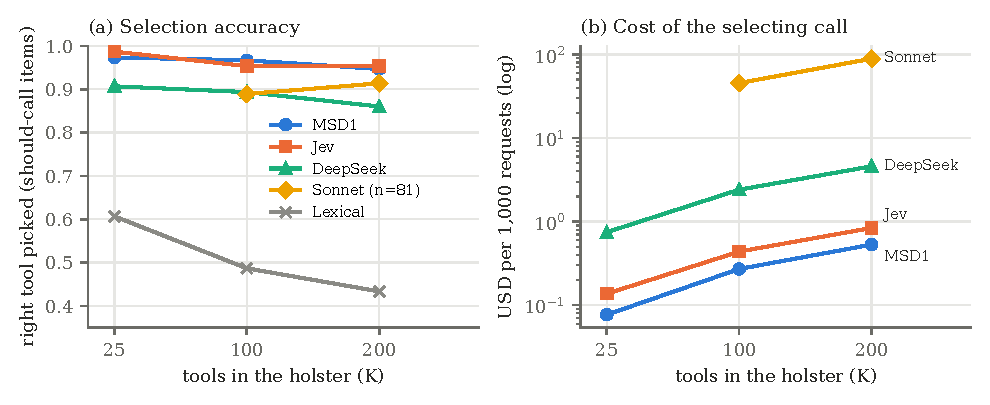
\includegraphics[width=\linewidth]{figures/fig_scaling.pdf}
\caption{Selection on BFCL items padded with random distractor tools. (a) Right tool chosen (should-call items;
$n=150$ per point; Sonnet on an 81-item subset at $K\ge100$). (b) Cost of the selecting call (log scale).}
\label{fig:scaling}
\end{figure}

\paragraph{Contamination-free selection.} On 288 items of a benchmark built on the day of the experiment
(fictional companies, tools in families of near-duplicate variants that differ in one implied detail, plus 28
coding-harness tools), with all 247 tools available, \msd{} chose correctly more often than DeepSeek ($p=0.024$)
and MiMo~V2.6~Pro ($p=3\times10^{-6}$) and tied GLM-5.3; its top three contained the right tool for every
should-call item.

\paragraph{Pre-registered coding-tool selection.} Before generating 86 fresh coding-harness items we recorded
hypotheses, metric (an acceptable next tool among 247) and test (exact McNemar, Holm over five comparisons); the
record is a local timestamped file, not an external registry. \msd{} chose an acceptable tool for 98.8\% of
items, Jev 90.7\%, against 77.9--88.4\% for three LLMs; all five hypotheses were supported (Holm $p\le0.035$).

\begin{table}[t]
\centering\small
\caption{Study 3: next-action agreement with resolved OpenHands trajectories (300 steps from 60 trajectories, one per repository). CIs resample whole trajectories. ``finish'': steps where the system predicted \texttt{finish} (3 of the 300 gold steps are \texttt{finish}).}
\label{tab:swe}
\begin{tabular}{@{}lrrrrr@{}}
\toprule
System & Agreement & 95\% CI & Top-2 & ``finish'' & \$/1k steps \\
\midrule
Always \texttt{execute\_bash} (majority) & 0.530 & 0.470--0.593 & -- & 0 & 0 \\
Repeat previous action & 0.410 & 0.360--0.467 & -- & 0 & 0 \\
Jev & \textbf{0.570} & 0.510--0.633 & 0.770 & 15 & 0.14 \\
Sonnet 5.5 & 0.533 & 0.473--0.597 & -- & 0 & 19.94 \\
DeepSeek & 0.527 & 0.470--0.587 & -- & 0 & 0.45 \\
\msd{} & 0.350 & 0.293--0.407 & 0.620 & 62 & 0.13 \\
\bottomrule
\end{tabular}
\end{table}


\end{document}
